
\section{Theorie}
\label{sec:Theorie}
Ein Laser (\textbf{L}ight \textbf{A}mplification by \textbf{S}timulated \textbf{E}mission of \textbf{R}adiation) ist eine Apparatur, die in der Lage ist
monochromatisches und kohärentes Licht mit hoher Intensität aus zu strahlen. Die drei wesentlichen Bauteile des Laser sind das sog. aktive Medium, die Pumpe sowie ein Resonator. \\
Im aktiven Medium entsteht die Laserstrahlung durch den Übergang von Elektronen in einen energetisch niederen Zustand unter Aussendung von Photonen.
Die Pumpe liefert die Energie, die nötig ist um eine Besetzungsinversion im aktiven Medium aufrecht zu erhalten. Besetzungsinversion bedeutet, dass sich mehr Teilchen in einem
energetisch ungünstigeren Zustand befinden als im energetisch günstigen.
Das letzte Bauteil, der Resonator, besteht aus zwei Spiegeln an denen die Photonen immer wieder reflektiert werden und so weitere Emissionen stimulieren können.
Die dadurch ausgelösten Photonen haben die oben genannten Eigenschaften.
\subsection{Stimulierte Emission}
Im Folgenden wird anhand eines 4-Niveau-Systems (siehe Abbildung (\ref{fig:4niv})) das Prinzip der stimulierten Emission erläutert.
\begin{figure}[h!]
  \centering
  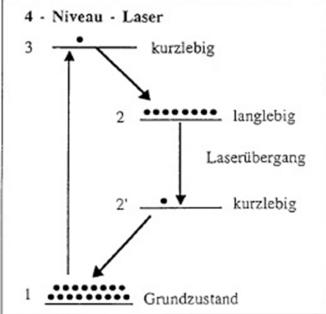
\includegraphics[scale=0.7]{fig/niveau.png}
  \caption{Beispiel für ein 4-Niveau-System \cite[6]{Anleitung3}.}
  \label{fig:4niv}
\end{figure}
\FloatBarrier
\noindent Dabei wird beispielsweie durch ein eingestrahltes Photon im Lasermedium ein Elektron mithilfe der Laserpumpe aus dem Grundzustand in einen angeregten, kurzlebigen Zustand versetzt und somit eine Besetzungsinversion erzeugt. Aus diesem Zustand fällt es schnell in einen langlebigen, stabilen und angeregten Zustand zurück. Dieser Zustand beschreibt das obere Laserniveau. Zwischen diesem oberen Laserniveau und dem unteren Laserniveau findet der Laserübergang statt. Die Energiedifferenz $\Delta E$ dieser beiden Niveaus
legt die Energie des Laserlichts fest. Fällt nun ein Photon mit genau der Energie $\Delta E$ ein, kann das Elektron vom oberen Laserniveau ins untere Laserniveau übergehen und dabei wird ein weiteres Photon
mit gleicher Phase, Energie und Richtung abgestrahlt. In Abbildung (\ref{fig:stimu}) ist dieser Vorgang schematisch dargestellt.
\begin{figure}[h!]
  \centering
  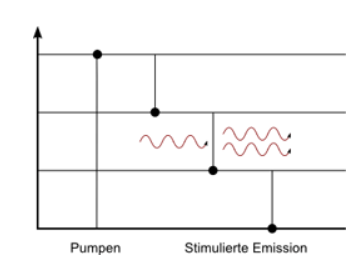
\includegraphics[scale=0.7]{fig/stimu.png}
  \caption{Schematische Darstellung von stimulierter Emission \cite{Anleitung10}.}
  \label{fig:stimu}
\end{figure}
\FloatBarrier
\subsection{Diodenlaser}
In diesem Versuch wird mit einem Galliumarsenid-Diodenlaser gearbeitet. Ein Diodenlaser besteht aus mindestens drei Schichten. Diese sind die n-Schicht, die aktive Schicht sowie die p-Schicht.
In Abbildung (\ref{fig:diod}) ist ein schematischer Laserchip dargestellt.
\begin{figure}[h!]
  \centering
  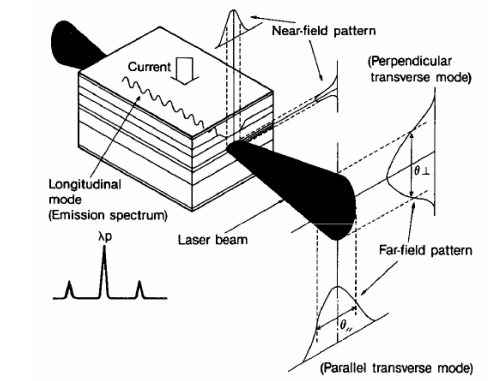
\includegraphics[scale=0.7]{fig/diod.png}
  \caption{Schematische Darstellung eines Diodenlaserchip \cite[3]{Anleitung}.}
  \label{fig:diod}
\end{figure}
\FloatBarrier
\noindent Die n- sowie die p-Schicht sind jeweils dotiert, sodass sie negativ mit Elektronen oder positiv mit sog. Elektronenlöchern geladen sind. Sobald jetzt ein Strom durch die Diode fließt, diffundieren sowohl Elektronen als auch Löcher in die aktive Schicht. Durch die Rekombination dieser wird ein Photon emittiert, ein weiteres Photon kann dabei für stimulierte Emission sorgen.
Dadurch, dass die Innenseiten der n-Schicht und der p-Schicht hochreflektiv sind, dienen diese als eine Art Kammer für die Photonen in der sich eine stehende Welle befindet.
Die dabei emittierte Strahlung kann dann durch die Front der Diode diese verlassen, da die Rückseite beinahe ideal reflektiv ist wird dort kaum Intensität verloren.\\

\noindent Damit die Diode in den Laserbetrieb kommt, ist es nötig einen Schwellenstrom zu erreichen, da unter diesem die Diode wie eine LED funktioniert. Dies liegt daran, dass erst ab einem bestimmten
Strom die Strahlung kohärent ist. Die dabei entstehende Strahlung ist divergent und im Gegensatz zu den atomaren Übergängen von einer großen Energiebandbreite. Damit dies nicht zum Problem
für den Diodenlaser wird, benutzt man die in Abbildung (\ref{fig:litt}) dargestellte Anordnung.
\begin{figure}[h!]
  \centering
  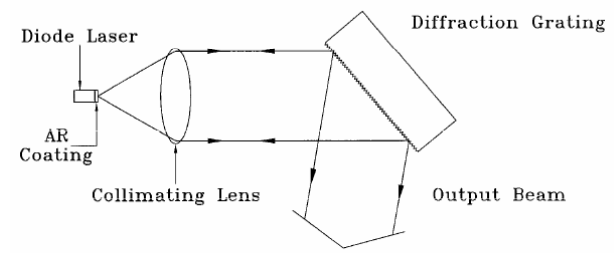
\includegraphics[scale=0.7]{fig/litt.png}
  \caption{Beispiel für die verwendete Anordnung \cite[5]{Anleitung}.}
  \label{fig:litt}
\end{figure}
\FloatBarrier
\noindent Die Linse richtet die divergente Strahlung zu einem parallelen Strahl. Durch das optische Gitter wird ein kleiner Teil der emittierten Strahlung zurück in die Diode reflektiert. Das Gitter sorgt ebenfalls dafür, dass keine externe Strahlung in die Diode gelangt. Dieser externe Hohlraum, der dadurch entsteht, hilft dabei die Laserstrahlung zu stabilisieren. Dadurch ist es möglich, eine wesentlich kleinere Energiebandbreite, als die der atomaren Übergänge, zu erzeugen.
\subsection{Einstellung des Diodenlasers}
In diesem Abschnitt wird darauf eingegangen wie die Frequenz des Diodenlasers zustande kommt. Diese wird durch mehrere Faktoren beeinflusst und ist die mit der höchsten optischen Zunahme. In Abbildung (\ref{fig:netga}) sind die verschiedenen Faktoren und deren Einflüsse in einer Grafik dargestellt.
\begin{figure}[h!]
  \centering
  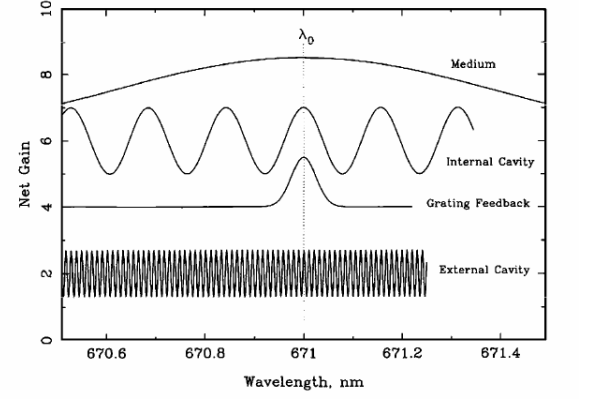
\includegraphics[scale=0.7]{fig/netga.png}
  \caption{Einflüsse auf die optische Zunahme durch verschiedene Faktoren aufgetragen gegen die Wellenlänge \cite[6]{Anleitung}.}
  \label{fig:netga}
\end{figure}
\FloatBarrier
\noindent Im Folgenden werden die einzelnen Einflüsse weiter erläutert.
\subsubsection{Medium}
Das Material aus dem die Laserdiode besteht hat den größten Einfluss auf die Wellenlänge mit der der Laser strahlt. Dieser Faktor kann einzig durch Erwärmung oder Abkühlung des Materials leicht
beeinflusst werden.
\subsubsection{Internal Cavity}
Die optische Zunahme, die durch den internen Hohlraum entsteht, wird von der Länge des Hohlraums und vom induzierten Strom festgelegt. Diese Zunahme ist periodisch, da in jedem optischen
Hohlraum eine Normal-Mode-Struktur vorliegt. Durch den induzierten Strom entsteht Wärme, die die Länge des Hohlraums verändert. Außerdem beeinflusst der Strom die Ladungskonzentration in
der aktiven Schicht des Laser. Dadurch, dass sowohl die optische Zunahme von Material, als auch die des inneren Hohlraums verschieden temperaturabhängig ist, kommt es zu sog. Modensprüngen zwischen
den Maxima der optischen Zunahme durch die innere Hohlkammer. Auf diese wird später noch explizit eingegangen.
\subsubsection{External Cavity}
Im Gegensatz zur internen Hohlkammer ist die externe Kammer, die aus dem optischen Gitter und der Rückseite der Laserdiode besteht, wesentlich größer. Daher ist wie in Abbildung (\ref{fig:netga}) zu sehen, die Periodendauer wesentlich kürzer.
\subsubsection{Grating Feedback}
Das optische Gitter reflektiert nur eine geringe Bandweite an Frequenzen zurück in die Diode, daher hat dieser Faktor nur einen einzelnen Peak in Abbildung (\ref{fig:netga}). Um den Peak zu verschieben,
wird der Winkel mit dem die Strahlung auf das optische Gitter trifft verändert.
\subsection{Modensprünge}
In diesem Theorieteil wird auf die oben genannten Modensprünge eingegangen. Diese entstehen durch das Zusammenspiel der einzelnen Faktoren auf die optische Zunahme. In Abbildung (\ref{fig:mode}) sind
diese dargestellt.
\begin{figure}[h!]
  \centering
  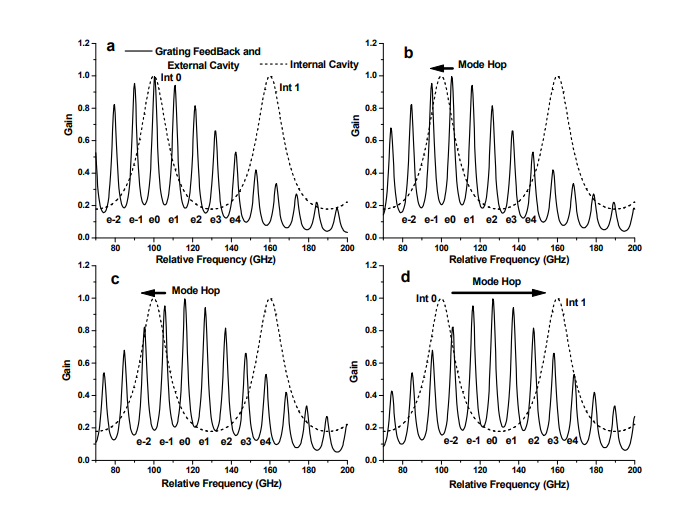
\includegraphics[scale=0.5]{fig/mode.png}
  \caption{Darstellung von Modensprüngen, ausgelöst durch Änderung des Gitterwinkel \cite[10]{Anleitung}.}
  \label{fig:mode}
\end{figure}
\FloatBarrier
\noindent Dadurch, dass durch Änderung des Gitterwinkel sich die maximale Zunahme des Grating-Feedbacks ändert und gleichzeitig auch durch die interne Hohlkammer, ist es möglich, dass die
emittierte Wellenlänge von einem Maximum der externen Hohlkammer zum nächsten Maximum springt (siehe Teil b in Abbildung (\ref{fig:mode})). Weiterhin ist es ebenfalls möglich, dass zu einem anderen Maximum der internen
Hohlkammer gesprungen wird (siehe Teil d in Abbildung (\ref{fig:mode})). Um diese Modensprünge zu verhindern wird die interne Hohlkammer simultan mit Veränderung des Gitterwinkels sowie Veränderung des Stromes angepasst.
